% LaTeX Template for Project Report, Version 2.0
% (Abstracted from a Major Project Report at CSED, NIT Calicut but can be
% modified easily to use for other reports also.)
%
% Released under Creative Commons Attribution license (CC-BY)
% Info: http://creativecommons.org/licenses/by/3.0/
%
% Created by: Kartik Singhal
% BTech CSE Batch of 2009-13
% NIT Calicut
% Contact Info: kartiksinghal@gmail.com
%
% It is advisable to learn the basics of LaTeX before using this template.
% A good resource to start with is http://en.wikibooks.org/wiki/LaTeX/
%
% All template fields are marked with a pair of angular brackets e.g. <title here>
% except for the ones defining citation names in ref.tex.
%
% Empty space after chapter/section/subsection titles can be used to insert text.
%
% Just compile this file using pdflatex after making all required changes.

\documentclass[12pt,a4paper]{report}
\usepackage{graphicx}
\usepackage{titlesec}
\setcounter{secnumdepth}{4}
\usepackage{url} %for proper url entries
\usepackage[bookmarks, colorlinks=false, pdfborder={0 0 0}, pdftitle={<pdf title here>}, pdfauthor={<author's name here>}, pdfsubject={<subject here>}, pdfkeywords={<keywords here>}]{hyperref} %for creating links in the pdf version and other additional pdf attributes, no effect on the printed document
%\usepackage[final]{pdfpages} %for embedding another pdf, remove if not required

\begin{document}
\renewcommand\bibname{References} %Renames "Bibliography" to "References" on ref page

%include other pages
\begin{titlepage}
	
	\begin{center}
		
		% Bottom of the page
		
\includegraphics[width=0.25\textwidth]{nitc-logo}\\[0.1in]
		\normalsize{Department of Computer Engineering and Information Technology}\\
		\normalsize
		\textsc{Amirkabir University of Technology}\\
		\vspace{0.5cm}
		
		
		\textup{\large {\sc B.Sc. Thesis}} %\small{Computer Engineering}}
		\\[0.4in]
		
		% Title
		\Large \textsc {Design and Implementation of a Real-Time Object Tracking system}\\[0.5in]
		
		\vspace{0.1in}
		\small \emph{Submitted in partial fulfillment of\\
			the degree}
		\vspace{.2in}
		
		{\sc Bachelor of Science \\in\\ Computer Engineering}\\[0.5in]
		
		\vspace{0.3in}
		% Submitted by
		\normalsize Submitted by\\
		\vspace{0.06in}
		\textsc{\large Sareh Soltani}
		
		\vspace{0.3in}
		% Submitted by
		\normalsize Conducted in\\
		\vspace{0.06in}
		\textsc{\small Aolab (The Academy for Amirkabir IoT Laboratory)}
		
		\vspace{.3in}
		Under the guidance of\\
		\vspace{0.06in}
		\textsc{\large Prof. Bahador Bakhshi}
		
		\vfill
		June 2019
				
	\end{center}	
\end{titlepage}
\vspace{2in}
\begin{abstract}
	In recent years, IoT technology has grown significantly and has been able to meet diverse and complex needs in various fields. One of the applications of the Internet of Things is real-time tracking. The positioning and tracking system has provided reliable solutions to ensure the safety of people and vehicles, and also has a significant impact on optimizing the quality of monitoring.  
	This system can be used for a broad range of applications such as traffic management and vehicle tracking/anti-theft system, and finally, traffic routing and navigation.  it can be applied in many business cases, like public transportation, so passengers can track their buses and trains by following the vehicle account on social networks.
	
	In this project, a system was developed to accurately determine the location, direction of movement, and speed of moving objects at any given time using SIM808 Module. In this system, each object is equipped with a GPS (Global Positioning System) module that receives its location every two minutes from the satellite and sends it to the software servers via the GSM modem. Software servers analyze the information after receiving it. In this part of the project, a web application was developed to process the transmitted data and then store it in a database and finally convert the stored information to visible to users. This allows you to see the speed, direction of movement, and the object's locations on the map. Furthermore, a heatmap was implemented to show the frequently visited places by users.
\end{abstract} 

\pagenumbering{roman} %numbering before main content starts
\tableofcontents
\listoffigures

\newpage
\pagenumbering{arabic} %reset numbering to normal for the main content

\chapter{Introduction}

In this section we'll take a brief look at the recent researches on \textit{Template Matching} task, its variants and the reliability of the models proposed in this task.
\section{Background and Recent Research}

\subsection{Feature Based Approach}
A featured-based approach is appropriate when both reference
and template images contain more correspondence
with respect to features and control points. In this case,
features include points, curves, or a surface model to perform
template matching. In this category, the final goal is to locate
the pair-wise connections between the target or so-called
reference and the template image using spatial relations
or features. In this approach, spatial relations, invariant
descriptors, pyramids, wavelets and relaxation methods play
an important role in extracting matching measures\cite{abstract}.

\subsection{Area Based Approach}
Area-based methods, which are usually known as correlation
methods or template matching, were developed for the
first time by Fonseca et al. [6] and are based on a combined
algorithm of feature detection and feature matching. This
method functions very well when the templates have no
strong features with an image, since they operate directly on
the pixel values. Matches are measured using the intensity
values of both image and template. The matching scores
are extracted by calculating squared differences in fixed
intensities, correction-based methods, optimization methods
and mutual information\cite{intro1}.

\subsection{Naive Template Matching}
Nave template matching is one of the basic methods of
extracting a given which is identical to the template from
the image target. In this approach, with or without scaling
(usually without scaling), the target image is scanned by the
template, and the similarity measures are calculated. Finally,
the positions with the strongest similarities are identified as
potential pattern positions\cite{abstract}. 

\subsection{Image Correlation Matching}
In this classic template matching method, the similarity
metric between the target and the template is measured.
Unlike the naive template matching algorithm, the target and the template might have different image intensities or
noise levels. However, those images must be aligned. The
similarity metric used in this approach is based on the
correlation between the target and the template\cite{intro2}.

\subsection{Sequential Similarity Detection Algorithms}
Sequential similarity detection algorithms (SSDAs) are
a more efficient alternative to correlation-based methods,
including matched filters for translational registration. The
measure of match is indirectly calculated based on an error
for corresponding pixels in f and g in the images under
comparison at any stage of the registration process\cite{intro3}.

\section{Motivation}
There are dozen optimized implementation of \textit{Template Matching} techniques, but the main motivation for me to do so, was the ability to model and code a real-life problem from scratch. I've also improved my CUDA and C++ programming skills with this project. Also, there are multiple math concepts covered in the \textit{Fast Fourier Transform} section which understanding them can bring an enhanced point of view in image and signal processing tasks. %literature survey included in this
\chapter{Tracking system components}
The main goal of our project is to design and implement a system that can determine the exact position of each moving object at any time. The mentioned system should be cost-effective in addition to proper performance.\\
To design such a system, we must first identify the system requirements and the overall architecture of the system we want. Then we use this architecture to implement the appropriate modules. In this chapter, in section 2.1, we first explain the general design of the tracking system and then in section 2.2, we introduce the components used in this design.

\section{System design and architecture}
In this section, we will design our system. According to the project's requirements, we must specify the transmitter and receiver modules, communication protocol, and application program for displaying information. The primary purpose of a tracking system is to track a specific object and gain its path. The tracking system provides information about the current location and speed of the object.\\
In this project, our communication has been one-way, in which the coordinates of the moving object are continuously measured and sent to a server. Then, the necessary processing of this information is performed on the server-side. According to the above explanations, we can mention three main parts in this system \cite{5}:
\begin{itemize}
	\item Obtain the location of a moving object using the GPS module
	\item Send location information to software servers by GSM modem
	\item Store location information on the server-side and implement an application to display the object's path on the map
\end{itemize}
As we have seen, the architecture of our system has four main parts. The first part is about locating the object from the satellite using the GPS module. The second part is related to sending the received information to the server using a GSM modem. The third part is the development of an application that uses the received data to display the location of the object on the map.\\
\begin{figure}[!h]
	\centerline{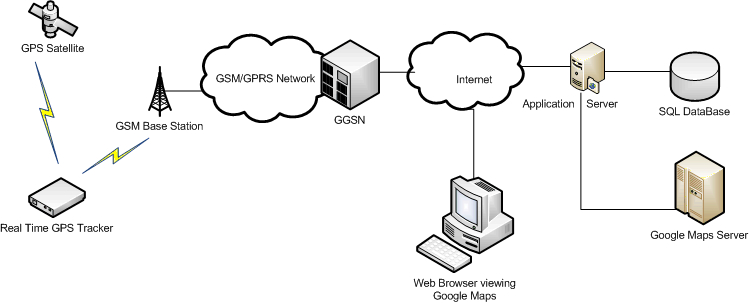
\includegraphics[width=.8\textwidth]{GPS_Tracker}}
	\caption{Block Diagram of Tracking System \cite{6}}
\end{figure}\\
Figure 2.1 shows an overview of the designed system architecture and the relationship between its parts. ّFor selecting the modules, it is necessary to know the task of each section accurately and choose the desired module for it \cite{7}.
\begin{itemize}
	\item In the first part, we need to measure the location of the object continuously. As soon as the object moves, the GPS module consistently receives the moving object's coordinate from the satellite. The signal received from the satellite is weak, so we must use an antenna to amplify the desired signal, and at the end, sends the amplified signal to the Arduino board.
	\item In the second part, the information received from the GPS module is sent to the server by the GSM modem.
	\item Software servers analyze the information after receiving them. Our communication in this project is one-way, and we will not have a request from software servers. In this part of the project, web-based software will be developed to process the submitted information and store them in the database. In the last section, this information will be displayed in the designed web page.
\end{itemize}
\begin{figure}[!h]
	\centerline{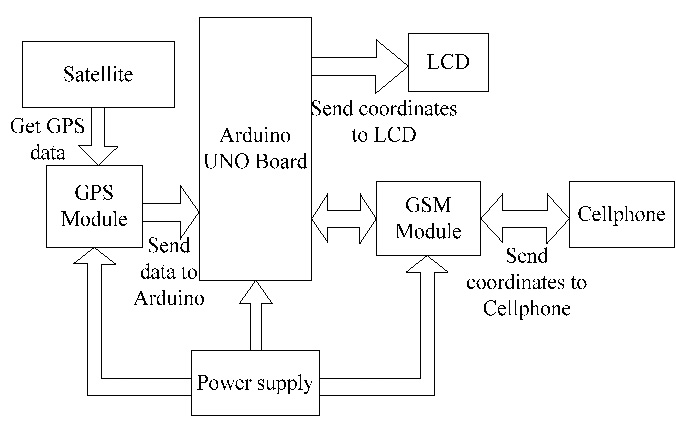
\includegraphics[width=.6\textwidth]{blockdiagram}}
	\caption{Architecture of Tracking System\cite{3}}
\end{figure}
\section{System components}
In the previous section, we defined the system architecture. Now we will express and introduce the components of this architecture in detail.
\subsection{Hardware components}
The hardware components used to implement this system are:
\begin{itemize}
	\item Arduino module
	\item SIM808 module
	\item GPS antenna
	\item GSM modem
\end{itemize}
\subsubsection{Arduino module}
Arduino is an open-source microprocessor suitable for writing applications that interact with the environment and objects outside. This board is ideal for prototyping, and its software and hardware design are freely available to all people. Any interested person, even with a little knowledge and experience in electronics, can use Arduino to do their projects.\\
Arduino has a simple programming environment that anyone with a little knowledge of C and C++ can program in this environment and run the program written in Arduino. Various sensors can be connected to the Arduino microcontroller and controlled. The microprocessor used on the Arduino board is based on the Arduino programming language and does not require any additional software or compiler for coding.\\
Figure 2.3 shows the Arduino Uno board:
\begin{figure}[!h]
	\centerline{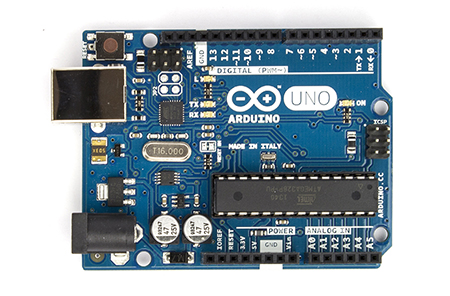
\includegraphics[width=.5\textwidth]{ArduinoUno_R3}}
	\caption{Arduino Uno board}
\end{figure}
\subsubsection{SIM808 module}
The 808 SIM module is a combination of GSM / GPS PRS 9 module and GPS module with 1900 MHz support for data transmission, SMS and voice calling.
This module has a SIM card socket in which the SIM card is inserted. Using the GSM / GPRS modem and the 808 SIM module, you can exchange data over the GSM network via the USB interface and access the information of devices located in remote locations.\\
In figure 2.4, You can see this chip.
\begin{figure}[!h]
	\centerline{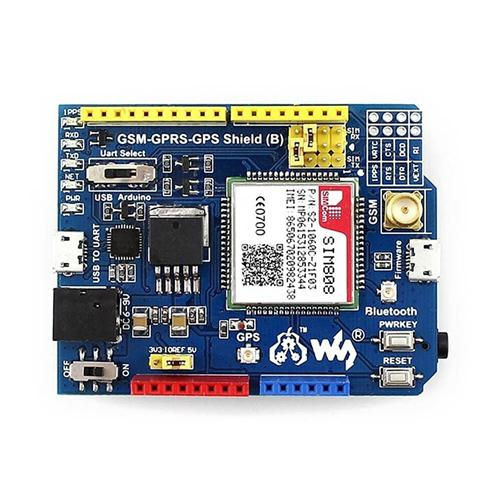
\includegraphics[width=.5\textwidth]{sim809}}
	\caption{SIM 808 module}
\end{figure}
\subsection{Software components}
\subsubsection{Arduino IDE}
The software used for programming is Arduino software, which you can see in Figure 2.5. Using the C language, you can write the required program, and after compiling, the generated hex code is uploaded on the Arduino. There are different libraries that make coding easier. The program is written using this software to receive data from satellite and send it to a mobile phone.\\
\begin{figure}[!h]
	\centerline{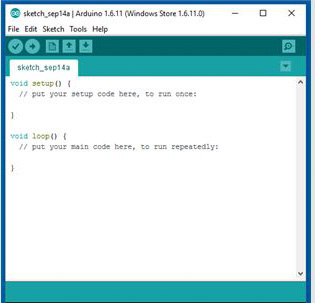
\includegraphics[width=.5\textwidth]{arduino-ide}}
	\caption{Arduino IDE}
\end{figure} %objective changed to problem definition
\chapter{Implementation and Performance Analysis}
In the previous section, we described the system's general architecture and the modules required to implement the tracking system. In this chapter, we will explain how the different parts are connected, and we will explain the implementation of the system.\\
The tracking system designed in this project uses Arduino module and the ُSIM 808, including the GSM and GPS antennas, for tracking. The core of this project is the Arduino microcontroller. The geographical location of object is received using a GPS antenna, and then this information is sent to the webserver using GSM technology. A web application has been developed to view and track an object on a map. This application consists of two parts: Front-end and Back-end. The front-end part has developed using Angular framework, and the Back-end part has developed using Express framework.\\
Initially, the SIM 808 module is initialized to get the location from the satellite. The initial settings of this device are done using AT commands. By connecting the GPS antenna, this module will be able to receive location coordinates from the satellite. Then the settings related to the GPRS network are done.\\
In fiqure 3.1 How to connect different modules in the tracking system is shown:\\
\begin{figure}[!h]
	\centerline{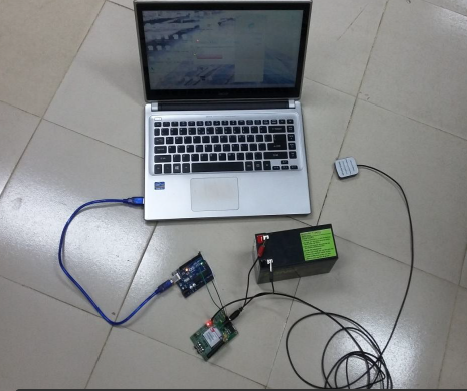
\includegraphics[width=.7\textwidth]{design-system}}
	\caption{Designed Tracking System}
\end{figure}\\
\section{Evaluate Tracking system performance}
As mentioned, the hardware part of our system consists of four modules, SIM 808, GSM receiver, GPS receiver, and Arduino microcontroller. This section will explain the implementation of the designed system, how to connect the various components and the implemented code.
\subsection{Circuit performance evaluation}
Before dealing with the modules and how to connect them, it is necessary to observe the system microcontroller performance and processing information in the flowchart. The overall performance of the system was described in the previous section. Now we have a flowchart about the implemented algorithm, and we can have a better understanding of the workflow in the hardware circuit designed and the code written for it.\\
The following diagram shows the general process of the implemented code on the Arduino.
\begin{figure}[h!]
	\centering
	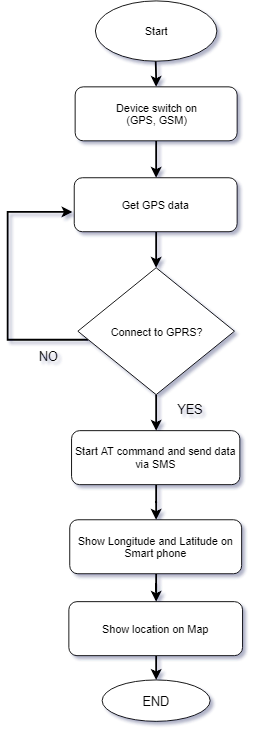
\includegraphics[width=.4\textwidth]{tracking-flowchart}
	\caption{Performance of implemented code on Arduino \cite{3}}
\end{figure}
\newpage
Firstly, for testing the system, the GPS antenna is connected to the SIM 808 module to receive the object's location (latitude and longitude) from the satellite. For doing this, the Arduino IDE software is used to program the code written on the Arduino board.\\
\newpage
The flowchart 3.3 shows how GPS works:\\
\begin{figure}[!h]
	\centerline{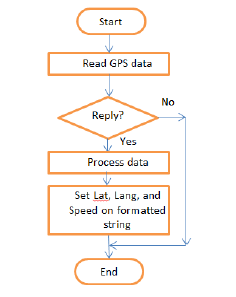
\includegraphics[width=.6\textwidth]{gps-flowchart}}
	\caption{Read Information diagram \cite{8}}
\end{figure}

For sending the object's location to the user via the GSM network, SIM 808 module and the Arduino microcontroller connected to it are used. For connecting 808 SIM module to the GSM network, we use AT commands to program and control it.\\
\newpage
The flowchart 3.4 shows how GSM works:\\
\begin{figure}[!h]
	\centerline{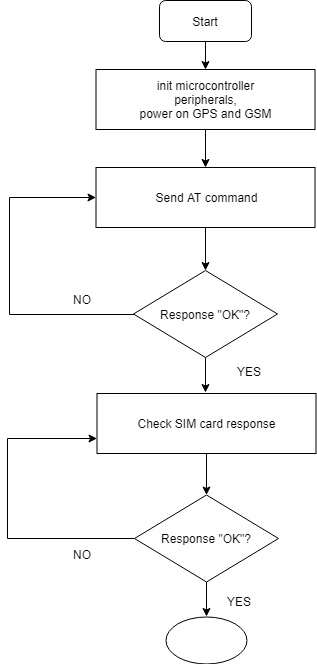
\includegraphics[width=.6\textwidth]{gsm-flowchart}}
	\caption{GSM \cite{8}}
\end{figure}
\newpage
\begin{figure}[!h]
	\centerline{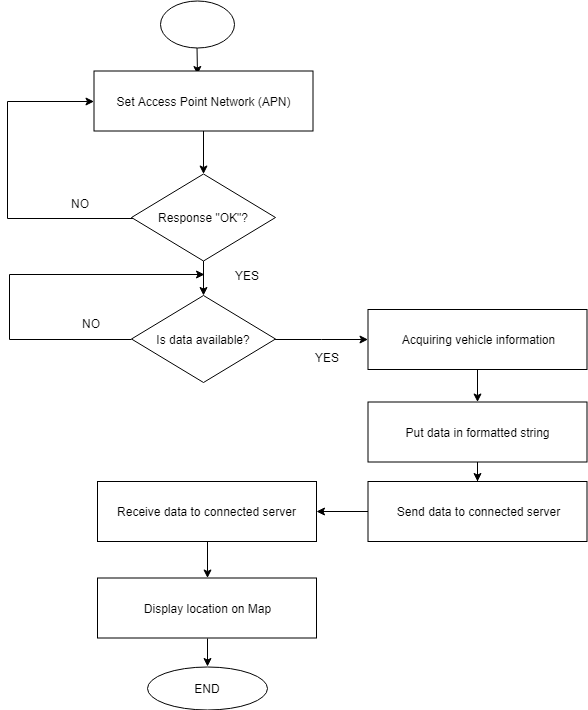
\includegraphics[width=.9\textwidth]{continue-gsm}}
	\caption{GSM \cite{8}}
\end{figure}
\chapter{Future Work}
We admit the possible drawbacks and inefficiencies existing in this project, thus we have the following key improvement to-do list:
\begin{itemize}
	\item Reorganization of the project structure, header files and .c files.
	\item Reorganization of the project source code for a C unified implementation.
	\item Usage shared memory techniques to improve the performance of the \textit{NTM} implementation.
	\item Usage of highly-optimized image libraries such as \textit{OpenCV} for \textit{image rotation}, \textit{image matrix extraction} and general \textit{bitmap processing}.
	\item Implementation of CUDA kernels for real-to-complex signal conversions.
	\item Implementation of CUDA kernel to find the number of occurrences of template signal in main signal in \textit{Fourier} based template matching.
\end{itemize}
\chapter{Conclusion}
In this project, we analyzed various algorithms for the task of \textit{Image Template Matching}. It is fair to say that there are already highly optimized libraries with template matching capabilities such as \textit{OpenCV}, but as mentioned before, the main purpose of this project is to improve the understanding of the CUDA environment and parallel implementation of highly-demanded computer vision tasks such as template matching.
We analyzed two main methods to perform this task:
\begin{enumerate}
	\item Naive Template Matching
	\item FFT Based Template Matching
\end{enumerate}
For further read, please refer to methods such as \textit{Stereo Matching}, \textit{Image Registration} and \textit{Scale Invariant Feature Transform}.
\cleardoublepage
%\pagebreak
\phantomsection
\addcontentsline{toc}{chapter}{References}
\begin{thebibliography}{99}
	
	\bibitem{1}M. Mukhtar, "\textit{{GPS} based Advanced Vehicle Tracking and Vehicle Control System,}" International Journal of Intelligent Systems and Applications, Feb. 2015.
	
	\bibitem{2}S. Hussain Shah and I. Yaqoob, "\textit{A survey: Internet of Things ({IOT}) technologies,  applications and challenges,}" 2016 {IEEE} Smart Energy Grid Engineering ({SEGE}), Aug. 2016.
	
	
	\bibitem{3}Md. Rahman, J.Mou, K. Tara and Md. Sarkar, "\textit{Real time Google map and Arduino based vehicle tracking system,}" 2016 {IEEE} Smart Energy Grid Engineering ({SEGE}), Aug. 2016.
	
	
	\bibitem{4}J. Saranya and J. Selvakumar, "\textit{Implementation of children tracking system on android mobile terminals,}" Implementation of children tracking system on android mobile terminals, Apr. 2013.
	
	\bibitem{5}B. Bidabad and A. Tayebi, "\textit{Design and implementation of vehicle tracking system using GPS/GSM/GPRS technology and smartphone application,}" 2014.
	
	\bibitem{6}M. Omar, H. Rashaand and T. Nicolae, "\textit{Design and implementation of real time tracking system based on Arduino Intel Galileo,}" 2016 8th International Conference on Electronics,  Computers and Artificial Intelligence ({ECAI}), Jun. 2016.

	\bibitem{7}T. Agrawal and M. Qadeer, "\textit{Tracing Path with Arduino Uno using {GPS} and {GPRS}/{GSM},}" 2018 International Conference on Computing,  Power and Communication Technologies ({GUCON}), Sep. 2018.
	
	\bibitem{8}A. ElShafee, M. Menshawi and M. Saeed, "\textit{Integrating Social Network Services with Vehicle Tracking Technologies,}" International Journal of Computer Applications, Jun. 2013.
	
	@article{ElShafee2013,
		doi = {10.5120/12539-9087},
		url = {https://doi.org/10.5120/12539-9087},
		year = {2013},
		month = jun,
		publisher = {Foundation of Computer Science},
		author = {Ahmed ElShafee and Mahmoud El Menshawi and Mena Saeed},
		title = {Integrating Social Network Services with Vehicle Tracking Technologies},
		journal = {International Journal of Computer Applications}
	}
	
\end{thebibliography}

\end{document}